%%
%% MScheme Numeric Tower: Module Abstraction Layers
%%
%% Companion to "Numeric Tower Phase 1: Implementation Proposal"
%%
\documentclass[12pt]{article}
\usepackage[margin=1in]{geometry}
\usepackage{booktabs}
\usepackage{listings}
\usepackage{xcolor}
\usepackage{hyperref}
\usepackage{textcomp}
\usepackage{amssymb}
\usepackage{amsmath}
\usepackage{enumitem}
\usepackage{longtable}
\usepackage{tikz}
\usetikzlibrary{arrows.meta,positioning,fit}

\lstdefinelanguage{Modula3}{
  morekeywords={MODULE,INTERFACE,IMPORT,FROM,PROCEDURE,BEGIN,END,
    VAR,CONST,TYPE,RECORD,OBJECT,METHODS,OVERRIDES,RETURN,
    IF,THEN,ELSE,ELSIF,WHILE,DO,FOR,TO,BY,LOOP,EXIT,REPEAT,UNTIL,
    CASE,OF,WITH,TRY,EXCEPT,FINALLY,RAISE,RAISES,
    NEW,ARRAY,REF,REFANY,SET,BOOLEAN,INTEGER,REAL,LONGREAL,EXTENDED,
    CHAR,TEXT,LONGINT,
    TRUE,FALSE,NIL,BRANDED,REVEAL,EVAL,NOT,AND,OR,IN,DIV,MOD,
    ISTYPE,NARROW,TYPECODE,GENERIC,ADDRESS,BITS,BITSIZE},
  sensitive=true,
  morecomment=[n]{(*}{*)},
  morestring=[b]",
}

\lstdefinelanguage{Scheme}{
  morekeywords={define,lambda,if,cond,else,let,let*,letrec,begin,
    set!,quote,exact?,inexact?,number?,integer?,real?,rational?,complex?,
    exact->inexact,inexact->exact,number->string,string->number,
    make-rectangular,make-polar,real-part,imag-part,magnitude,angle,
    numerator,denominator,rationalize},
  sensitive=true,
  morecomment=[l]{;},
  morestring=[b]",
  literate={lambda}{$\lambda$}1,
}

\lstset{
  basicstyle=\ttfamily\small,
  breaklines=true,
  frame=single,
  backgroundcolor=\color{gray!5},
  keywordstyle=\bfseries\color{blue!70!black},
  commentstyle=\itshape\color{green!50!black},
  stringstyle=\color{red!60!black},
  showstringspaces=false,
  columns=flexible,
  tabsize=2,
  xleftmargin=2em,
  framexleftmargin=1.5em,
}

\title{\bfseries\sffamily\fontsize{24.88}{30}\selectfont
  Numeric Tower Abstraction Layers}
\author{Mika Nystr\"om \\ {\tt mika@alum.mit.edu}}
\date{March 2026}

\begin{document}
\maketitle
\thispagestyle{empty}

\newpage
\tableofcontents
\newpage

%======================================================================
\section{Motivation}
\label{sec:motivation}
%======================================================================

After Phase~1 of the numeric tower implementation, {\tt Mpz.T}
references leaked throughout MScheme's core modules.  The
interpreter's use of {\tt Mpz.T} as its bignum representation is
an implementation detail---it happens to coincide with
{\tt cspgrammar}/{\tt cspsimlib} using {\tt Mpz.T} as a
computation type, but these are independent choices.  Similarly,
{\tt SchemeLongReal.T} is a specific representation (boxed IEEE~754
{\tt LONGREAL}) that could be replaced or supplemented by
{\tt SchemeMpfr.T} for configurable-precision arithmetic.

This document defines a set of abstraction modules that cleanly
layer the numeric tower, hiding representation details from most
of the codebase and providing a stable Modula-3 API for clients.
The design accommodates the full R5RS numeric tower:
\[
  \mathit{number} \supset \mathit{complex} \supset \mathit{real}
  \supset \mathit{rational} \supset \mathit{integer}
\]
even though only integer and real (inexact) types are implemented
in Phase~1.

%======================================================================
\section{The R5RS Numeric Tower}
\label{sec:r5rs-tower}
%======================================================================

R5RS defines five numeric types forming a subtype chain, crossed
with an orthogonal exactness dimension:

\begin{center}
\begin{tabular}{lcc}
\toprule
\textbf{Type} & \textbf{Exact} & \textbf{Inexact} \\
\midrule
integer   & fixnum, bignum ({\tt Mpz.T}) & {\tt SchemeLongReal.T} with integer value \\
rational  & {\tt Mpq.T} (future) & {\tt SchemeLongReal.T} \\
real      & (= rational when exact) & {\tt SchemeLongReal.T}, {\tt SchemeMpfr.T} (future) \\
complex   & pair of exact reals (future) & pair of inexact reals (future) \\
number    & \multicolumn{2}{c}{union of the above} \\
\bottomrule
\end{tabular}
\end{center}

\paragraph{Key distinctions.}
\begin{itemize}[nosep]
\item \emph{Exactness} is a property of a value, not a type.
  {\tt 3} is an exact integer; {\tt 3.0} is an inexact integer.
  They are {\tt equal?}\ but not {\tt eqv?}.
\item Every exact integer is an exact rational (with denominator~1).
\item Every exact rational is a real.  There are no irrational exact
  reals in R5RS (no symbolic $\sqrt{2}$).
\item Complex numbers have real and imaginary parts, each of which
  may be exact or inexact.
\end{itemize}

%======================================================================
\section{Concrete Representations}
\label{sec:representations}
%======================================================================

Table~\ref{tab:repr} enumerates all concrete Modula-3 types used
(or planned) to represent Scheme numeric values.

\begin{table}[htbp]
\centering
\begin{tabular}{llll}
\toprule
\textbf{M3 Type} & \textbf{Scheme Tower Level} & \textbf{Exactness} & \textbf{Status} \\
\midrule
{\tt SchemeInt.T} ({\tt REF INTEGER}) & integer & exact & Phase~1 \\
{\tt Mpz.T} & integer & exact & Phase~1 \\
{\tt Mpq.T} & rational & exact & Phase~2 (future) \\
{\tt SchemeLongReal.T} ({\tt REF LONGREAL}) & real & inexact & Phase~1 \\
{\tt SchemeMpfr.T} & real & inexact & Phase~5 (future) \\
{\tt SchemeComplex.T} & complex & either & Phase~3 (future) \\
\bottomrule
\end{tabular}
\caption{Concrete representations for numeric values.}
\label{tab:repr}
\end{table}

\paragraph{{\tt Mpq.T} (exact rational).}
GMP provides {\tt mpq\_t}, an exact rational type stored as a
pair of {\tt mpz\_t} values (numerator and denominator) in
canonical form (coprime, positive denominator).  A Modula-3
binding {\tt Mpq} would follow the same pattern as {\tt Mpz}.
Exact rationals arise from:
\begin{itemize}[nosep]
\item Exact division: {\tt (/ 1 3)} $\to$ $\frac{1}{3}$
  (currently returns inexact {\tt 0.333...})
\item {\tt rationalize}: {\tt (rationalize 3.14 0.01)} $\to$ $\frac{22}{7}$
\item Arithmetic on rationals: {\tt (+ 1/3 1/6)} $\to$ $\frac{1}{2}$
\end{itemize}
An exact integer is a rational with denominator~1.  The
implementation should recognize this case and store as
{\tt SchemeInt.T} or {\tt Mpz.T} rather than {\tt Mpq.T},
avoiding unnecessary overhead.

\paragraph{{\tt SchemeMpfr.T} (arbitrary-precision inexact).}
MPFR provides correctly-rounded arbitrary-precision floating-point
arithmetic.  {\tt SchemeMpfr.T} would be a boxed MPFR value with
a configurable precision parameter.  The default precision could
match {\tt LONGREAL} (53~bits), with a Scheme-accessible
procedure to change it.  MPFR depends on GMP, so enabling MPFR
implies GMP is available.

\paragraph{{\tt SchemeComplex.T} (complex numbers).}
A complex number is a pair of real parts.  Two representations
are natural:
\begin{enumerate}[nosep]
\item \emph{Rectangular}: real part + imaginary part, both
  {\tt SchemeObject.T} (can be exact or inexact).
\item \emph{Polar}: magnitude + angle, always inexact (since
  angles involve transcendentals).
\end{enumerate}
The rectangular form is canonical for storage; polar is a
conversion.  A complex number with zero imaginary part should
be automatically demoted to a real (just as a bignum that fits
in a fixnum is demoted).

%======================================================================
\section{Module Hierarchy}
\label{sec:hierarchy}
%======================================================================

The numeric tower is organized in layers, from most specific
(representation-aware) to most abstract (representation-free).

\begin{center}
\begin{tabular}{clp{7cm}}
\toprule
\textbf{Layer} & \textbf{Module} & \textbf{Responsibility} \\
\midrule
4 & {\tt SchemeNumber} & Full-tower dispatch across all types,
  including complex.  The ``one-stop'' API for generic numeric
  operations on {\tt SchemeObject.T} values. \\[4pt]
3 & {\tt SchemeExact} & Exact-number abstraction: integer (fixnum +
  bignum) and rational ({\tt Mpq.T}).  Hides {\tt Mpz.T} and
  {\tt Mpq.T} from callers. \\[4pt]
3 & {\tt SchemeInexact} & Inexact-number abstraction: currently
  {\tt SchemeLongReal.T}; extensible to {\tt SchemeMpfr.T}.
  Hides the specific floating-point representation. \\[4pt]
3 & {\tt SchemeComplex} & Complex-number operations: construction,
  {\tt real-part}, {\tt imag-part}, {\tt magnitude}, {\tt angle}.
  Dispatches component operations to {\tt SchemeExact}/{\tt
  SchemeInexact}. \\[4pt]
2 & {\tt SchemeInt} & Fixnum representation: {\tt REF INTEGER},
  cache, overflow-safe {\tt INTEGER} arithmetic that promotes
  to {\tt Mpz.T}.  Also exports {\tt ToMpz}/{\tt MpzToScheme}
  for the interop boundary. \\[4pt]
2 & {\tt SchemeLongReal} & Inexact representation: {\tt REF
  LONGREAL}, common constants, {\tt FromO}/{\tt Int} conversion. \\[4pt]
1 & {\tt Mpz} & GMP bignum bindings. \\[4pt]
1 & {\tt Mpq} & GMP rational bindings (future). \\[4pt]
1 & {\tt Mpfr} & MPFR arbitrary-precision float bindings (future). \\[4pt]
1 & {\tt SchemePrimitive} & Numeric engine: bitwise operations,
  {\tt gcd}/{\tt lcm}, {\tt expt}, {\tt number->string}, etc. \\
\bottomrule
\end{tabular}
\end{center}

\paragraph{Key invariant.}
Modules at Layer~3 and above do \emph{not} import {\tt Mpz},
{\tt Mpq}, or {\tt Mpfr}.  They operate exclusively through
{\tt SchemeObject.T} values and delegate to Layer~2 modules for
representation-specific work.

%----------------------------------------------------------------------
\subsection{Dependency Diagram}
%----------------------------------------------------------------------

\begin{center}
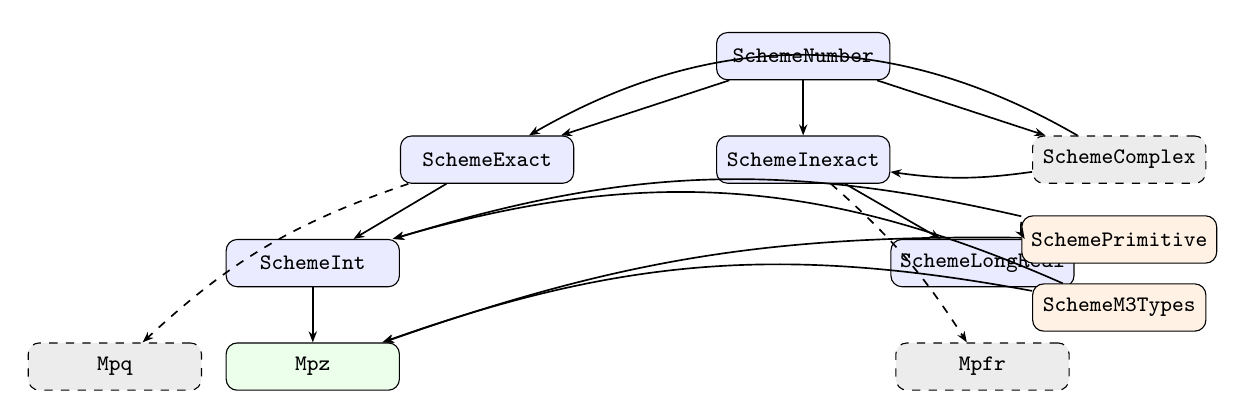
\begin{tikzpicture}[
  mod/.style={draw, rounded corners, fill=blue!8, minimum width=2.2cm,
              minimum height=0.6cm, font=\footnotesize\tt},
  future/.style={mod, fill=gray!15, dashed},
  engine/.style={mod, fill=orange!10},
  lib/.style={mod, fill=green!8},
  arr/.style={-{Stealth[length=4pt]}, semithick},
  node distance=0.5cm and 0.8cm
]

% Layer 4
\node[mod] (snum) {SchemeNumber};

% Layer 3 — compact horizontal spread
\node[mod, below left=0.7cm and 1.8cm of snum] (sexact) {SchemeExact};
\node[mod, below=0.7cm of snum] (sinexact) {SchemeInexact};
\node[future, below right=0.7cm and 1.8cm of snum] (scomplex) {SchemeComplex};

% Layer 2
\node[mod, below left=0.7cm and 0cm of sexact] (sint) {SchemeInt};
\node[mod, below right=0.7cm and 0cm of sinexact] (slr) {SchemeLongReal};

% Layer 1 — tight row
\node[lib, below=0.7cm of sint] (mpz) {Mpz};
\node[future, left=0.3cm of mpz] (mpq) {Mpq};
\node[future, below=0.7cm of slr] (mpfr) {Mpfr};

% Engine — below SchemeComplex to avoid width overflow
\node[engine, below=0.4cm of scomplex] (sprim) {\footnotesize SchemePrimitive};
\node[engine, below=0.25cm of sprim] (smt) {\footnotesize SchemeM3Types};

% Arrows - Layer 4 to 3
\draw[arr] (snum) -- (sexact);
\draw[arr] (snum) -- (sinexact);
\draw[arr] (snum) -- (scomplex);

% Arrows - Layer 3 to 2
\draw[arr] (sexact) -- (sint);
\draw[arr] (sinexact) -- (slr);
\draw[arr] (scomplex) to[bend left=8] (sinexact);
\draw[arr] (scomplex) to[bend right=30] (sexact);

% Arrows - Layer 2 to 1
\draw[arr] (sint) -- (mpz);
\draw[arr, dashed] (sexact) to[bend right=12] (mpq);
\draw[arr, dashed] (sinexact) to[bend left=8] (mpfr);

% Engine arrows
\draw[arr] (sprim) to[bend right=15] (sint);
\draw[arr] (sprim) to[bend right=10] (mpz);
\draw[arr] (sprim) to[bend right=20] (slr);
\draw[arr] (smt) to[bend right=20] (sint);
\draw[arr] (smt) to[bend right=15] (mpz);

\end{tikzpicture}
\end{center}

\noindent Solid boxes are Phase~1 (current); dashed boxes are
future phases.  {\tt SchemePrimitive} and {\tt SchemeModula3Types}
(orange) are ``engine'' modules that legitimately import
representation types directly.

%======================================================================
\section{New Interfaces}
\label{sec:interfaces}
%======================================================================

%----------------------------------------------------------------------
\subsection{{\tt SchemeExact}}
\label{sec:iface-exact}
%----------------------------------------------------------------------

The exact-number abstraction.  In Phase~1, operates on fixnums
({\tt REF INTEGER}) and bignums ({\tt Mpz.T}).  In Phase~2, will
also handle exact rationals ({\tt Mpq.T}).

\begin{lstlisting}[language=Modula3]
INTERFACE SchemeExact;
IMPORT SchemeObject;

(* Predicate *)
PROCEDURE Is(x: SchemeObject.T): BOOLEAN;
  (* TRUE iff x is an exact number.
     Phase 1: fixnum or bignum.
     Phase 2: also exact rational. *)

PROCEDURE IsInteger(x: SchemeObject.T): BOOLEAN;
  (* TRUE iff x is an exact integer (not a non-integer rational) *)

(* Sign predicates --- checked runtime error if not exact *)
PROCEDURE IsZero(x: SchemeObject.T): BOOLEAN;
PROCEDURE IsPositive(x: SchemeObject.T): BOOLEAN;
PROCEDURE IsNegative(x: SchemeObject.T): BOOLEAN;

(* Arithmetic --- operands must be exact.
   Phase 1: integer arithmetic.
   Phase 2: rational arithmetic (Div returns exact rational
   when remainder is non-zero). *)
PROCEDURE Add(a, b: SchemeObject.T): SchemeObject.T;
PROCEDURE Sub(a, b: SchemeObject.T): SchemeObject.T;
PROCEDURE Mul(a, b: SchemeObject.T): SchemeObject.T;
PROCEDURE Div(a, b: SchemeObject.T): SchemeObject.T;
  (* Phase 1: truncated quotient (integer division).
     Phase 2: exact rational division (1/3 -> Mpq.T). *)
PROCEDURE Rem(a, b: SchemeObject.T): SchemeObject.T;
  (* Truncated remainder.  Integer operands only. *)
PROCEDURE Neg(a: SchemeObject.T): SchemeObject.T;
PROCEDURE Abs(a: SchemeObject.T): SchemeObject.T;

(* Comparison --- operands must be exact *)
PROCEDURE Compare(a, b: SchemeObject.T): INTEGER;
  (* Returns -1, 0, or 1.
     Phase 2: handles rational vs integer comparison. *)

(* Conversion *)
PROCEDURE ToInteger(x: SchemeObject.T): INTEGER;
  (* Checked runtime error if not exact integer or out of range.
     Phase 2: error if rational with denominator > 1. *)
PROCEDURE ToLongReal(x: SchemeObject.T): LONGREAL;
  (* Exact -> LONGREAL (may lose precision for large values) *)
PROCEDURE Format(x: SchemeObject.T): TEXT;
  (* Phase 1: decimal integer.
     Phase 2: "n/d" for non-integer rationals. *)

(* Phase 2 additions *)
(* PROCEDURE Numerator(x: SchemeObject.T): SchemeObject.T; *)
(* PROCEDURE Denominator(x: SchemeObject.T): SchemeObject.T; *)

(* Construction *)
PROCEDURE FromI(x: INTEGER): SchemeObject.T;
  (* Convenience: delegates to SchemeInt.FromI *)

VAR (* CONST, set in module body *)
  Zero, One, NegOne, Two: SchemeObject.T;

END SchemeExact.
\end{lstlisting}

\paragraph{Phase~2 evolution (exact rationals).}
When {\tt Mpq.T} is added:
\begin{itemize}[nosep]
\item {\tt Is} returns {\tt TRUE} for {\tt Mpq.T} values.
\item {\tt IsInteger} distinguishes integers from non-integer
  rationals (checks denominator = 1).
\item {\tt Div} returns an exact rational ({\tt Mpq.T}) when the
  division is not exact, instead of falling through to inexact.
  Example: {\tt (/ 1 3)} $\to$ {\tt Mpq.T} representing $\frac{1}{3}$.
\item {\tt Rem} continues to require integer operands.
\item {\tt Compare} handles rational$\times$integer and
  rational$\times$rational via {\tt mpq\_cmp}.
\item {\tt Format} returns {\tt "1/3"} for rationals.
\item {\tt Numerator}/{\tt Denominator} are added.
\item Results are automatically simplified: a rational with
  denominator~1 is demoted to an integer, just as a bignum that
  fits in a fixnum is demoted.
\end{itemize}

\paragraph{Relationship to {\tt SchemeInt}.}
{\tt SchemeInt} remains the fixnum-level module.  Its
{\tt Add}/{\tt Sub}/{\tt Mul} take {\tt INTEGER} operands (the
fast path when both operands are known fixnums).
{\tt SchemeExact.Add}/etc.\ take {\tt SchemeObject.T} operands
and dispatch across all combinations.
{\tt SchemeInt.ToMpz} and {\tt SchemeInt.MpzToScheme} remain
exported from {\tt SchemeInt} for use by {\tt SchemePrimitive}
and {\tt SchemeModula3Types}, but are \emph{not} part of the
{\tt SchemeExact} abstraction.

%----------------------------------------------------------------------
\subsection{{\tt SchemeInexact}}
\label{sec:iface-inexact}
%----------------------------------------------------------------------

The inexact-number abstraction.  Currently wraps
{\tt SchemeLongReal.T}; designed to accommodate {\tt SchemeMpfr.T}
without changing callers.

\begin{lstlisting}[language=Modula3]
INTERFACE SchemeInexact;
IMPORT SchemeObject;

(* Predicate *)
PROCEDURE Is(x: SchemeObject.T): BOOLEAN;
  (* TRUE iff x is an inexact number.
     Phase 1: SchemeLongReal.T.
     Phase 5: also SchemeMpfr.T. *)

(* Arithmetic --- operands must be inexact *)
PROCEDURE Add(a, b: SchemeObject.T): SchemeObject.T;
PROCEDURE Sub(a, b: SchemeObject.T): SchemeObject.T;
PROCEDURE Mul(a, b: SchemeObject.T): SchemeObject.T;
PROCEDURE Div(a, b: SchemeObject.T): SchemeObject.T;
PROCEDURE Neg(a: SchemeObject.T): SchemeObject.T;
PROCEDURE Abs(a: SchemeObject.T): SchemeObject.T;

(* Comparison --- operands must be inexact *)
PROCEDURE Compare(a, b: SchemeObject.T): INTEGER;

(* Conversion *)
PROCEDURE ToLongReal(x: SchemeObject.T): LONGREAL;
  (* Phase 5: SchemeMpfr.T -> LONGREAL with possible precision loss *)
PROCEDURE FromLongReal(x: LONGREAL): SchemeObject.T;
PROCEDURE FromInteger(x: INTEGER): SchemeObject.T;
PROCEDURE Format(x: SchemeObject.T): TEXT;
  (* Ensures decimal point in output for distinguishability *)

END SchemeInexact.
\end{lstlisting}

\paragraph{Phase~5 evolution (MPFR).}
When {\tt SchemeMpfr.T} is added:
\begin{itemize}[nosep]
\item {\tt Is} returns {\tt TRUE} for both {\tt SchemeLongReal.T}
  and {\tt SchemeMpfr.T}.
\item Arithmetic between two {\tt SchemeLongReal.T} values uses
  hardware {\tt LONGREAL} (fast path).  Arithmetic involving
  {\tt SchemeMpfr.T} uses MPFR (precision contagion: the result
  inherits the higher precision).
\item {\tt ToLongReal} downconverts {\tt SchemeMpfr.T} to 64-bit
  with possible precision loss.
\item A new {\tt FromMpfr}/{\tt ToMpfr} pair would be added for
  explicit MPFR construction.
\item {\tt Format} for {\tt SchemeMpfr.T} prints all significant
  digits at the value's precision.
\end{itemize}

\paragraph{Two-tier inexact precision.}
An interesting design question is whether {\tt SchemeLongReal.T}
and {\tt SchemeMpfr.T} should coexist or whether MPFR should
replace {\tt LONGREAL} entirely.  Arguments for coexistence:
\begin{itemize}[nosep]
\item Hardware {\tt LONGREAL} is 5--50$\times$ faster than MPFR
  at the same precision.  Most programs don't need extra precision.
\item The compiler's self-tail-call optimization unboxes to
  {\tt LONGREAL}.  Replacing with MPFR would require a different
  unboxing strategy.
\item Existing M3 code that calls {\tt SchemeLongReal.FromO} to
  extract a {\tt LONGREAL} would need no changes.
\end{itemize}
Arguments for replacement:
\begin{itemize}[nosep]
\item Simpler---only one inexact representation to dispatch on.
\item MPFR at 53-bit precision gives identical results to
  {\tt LONGREAL} (correctly rounded).
\item Eliminates the question of what happens when a
  {\tt SchemeLongReal.T} and a {\tt SchemeMpfr.T} are combined.
\end{itemize}
The {\tt SchemeInexact} abstraction supports either choice
transparently.

%----------------------------------------------------------------------
\subsection{{\tt SchemeComplex} (Phase~3)}
\label{sec:iface-complex}
%----------------------------------------------------------------------

Complex number support.  A {\tt SchemeComplex.T} stores a pair
of real-valued {\tt SchemeObject.T} values (real part and
imaginary part), each of which may be exact or inexact.

\begin{lstlisting}[language=Modula3]
INTERFACE SchemeComplex;
IMPORT SchemeObject;
FROM Scheme IMPORT E;

TYPE T <: SchemeObject.T;

(* Predicate *)
PROCEDURE Is(x: SchemeObject.T): BOOLEAN;
  (* TRUE iff x is a complex number (with non-zero imaginary part).
     Note: real numbers are trivially complex but are NOT
     represented as SchemeComplex.T. *)

(* Construction *)
PROCEDURE MakeRectangular(re, im: SchemeObject.T): SchemeObject.T
  RAISES {E};
  (* If im is zero, returns re directly (demotion to real). *)

PROCEDURE MakePolar(mag, angle: SchemeObject.T): SchemeObject.T
  RAISES {E};
  (* Converts to rectangular form internally. *)

(* Accessors *)
PROCEDURE RealPart(x: SchemeObject.T): SchemeObject.T;
  (* For non-complex numbers, returns x itself. *)
PROCEDURE ImagPart(x: SchemeObject.T): SchemeObject.T;
  (* For non-complex numbers, returns exact zero. *)
PROCEDURE Magnitude(x: SchemeObject.T): SchemeObject.T
  RAISES {E};
PROCEDURE Angle(x: SchemeObject.T): SchemeObject.T
  RAISES {E};

(* Arithmetic *)
PROCEDURE Add(a, b: SchemeObject.T): SchemeObject.T RAISES {E};
PROCEDURE Sub(a, b: SchemeObject.T): SchemeObject.T RAISES {E};
PROCEDURE Mul(a, b: SchemeObject.T): SchemeObject.T RAISES {E};
PROCEDURE Div(a, b: SchemeObject.T): SchemeObject.T RAISES {E};
PROCEDURE Neg(a: SchemeObject.T): SchemeObject.T RAISES {E};

(* Formatting *)
PROCEDURE Format(x: SchemeObject.T): TEXT;
  (* "a+bi" or "a-bi" form *)

END SchemeComplex.
\end{lstlisting}

\paragraph{Design decisions.}
\begin{itemize}
\item \textbf{Demotion}: {\tt MakeRectangular(3, 0)} returns
  {\tt SchemeInt.FromI(3)}, not a complex with zero imaginary part.
  This ensures that {\tt (real? (make-rectangular 3 0))} returns
  {\tt \#t} as R5RS requires.
\item \textbf{Exactness}: A complex number {\tt 3+4i} where both
  parts are exact is itself exact.  {\tt (exact? 3+4i)} $\to$ {\tt \#t}.
  If either part is inexact, the complex is inexact.
\item \textbf{Mixed arithmetic}: {\tt (+ 3+4i 2.0)} involves an
  inexact real and an exact complex.  The real is promoted to
  complex {\tt 2.0+0.0i}, and the result is inexact complex
  {\tt 5.0+4.0i} (double contagion: inexactness \emph{and}
  complexness propagate).
\item \textbf{Transcendentals}: {\tt (sqrt -1)} $\to$ {\tt 0+1i}
  requires complex results from real arguments.  This is a
  ``complexness promotion'' triggered by the operation, not by
  the operand types.
\end{itemize}

%----------------------------------------------------------------------
\subsection{{\tt SchemeNumber}}
\label{sec:iface-number}
%----------------------------------------------------------------------

The full numeric tower.  Dispatches across exact, inexact, and
complex types.  Implements exactness contagion and complex
promotion.

\begin{lstlisting}[language=Modula3]
INTERFACE SchemeNumber;
IMPORT SchemeObject;
FROM Scheme IMPORT E;

(* Predicates *)
PROCEDURE Is(x: SchemeObject.T): BOOLEAN;
  (* TRUE for any number: exact, inexact, or complex *)

PROCEDURE IsExact(x: SchemeObject.T): BOOLEAN;
  (* TRUE for exact numbers (integer, rational, exact complex) *)

PROCEDURE IsInexact(x: SchemeObject.T): BOOLEAN;
  (* TRUE for inexact numbers *)

(* Full-tower arithmetic: handles all combinations *)
PROCEDURE Add(a, b: SchemeObject.T): SchemeObject.T RAISES {E};
PROCEDURE Sub(a, b: SchemeObject.T): SchemeObject.T RAISES {E};
PROCEDURE Mul(a, b: SchemeObject.T): SchemeObject.T RAISES {E};
PROCEDURE Div(a, b: SchemeObject.T): SchemeObject.T RAISES {E};
PROCEDURE Neg(a: SchemeObject.T): SchemeObject.T RAISES {E};
PROCEDURE Abs(a: SchemeObject.T): SchemeObject.T RAISES {E};

(* Full-tower comparison *)
PROCEDURE Compare(a, b: SchemeObject.T): INTEGER RAISES {E};
  (* Defined only for real numbers; error on complex *)
PROCEDURE Equal(a, b: SchemeObject.T): BOOLEAN RAISES {E};
  (* Numeric equality across the full tower *)

(* Conversion *)
PROCEDURE ToLongReal(x: SchemeObject.T): LONGREAL RAISES {E};
  (* Error on complex *)
PROCEDURE ToInteger(x: SchemeObject.T): INTEGER RAISES {E};
  (* Error on complex, non-integer rational, or out-of-range *)
PROCEDURE ExactToInexact(x: SchemeObject.T): SchemeObject.T
  RAISES {E};
PROCEDURE InexactToExact(x: SchemeObject.T): SchemeObject.T
  RAISES {E};

(* Formatting *)
PROCEDURE Format(x: SchemeObject.T): TEXT;
  (* Dispatches to SchemeExact.Format, SchemeInexact.Format,
     or SchemeComplex.Format as appropriate *)

END SchemeNumber.
\end{lstlisting}

\paragraph{Dispatch rules.}
For a binary operation {\tt op(a, b)}:
\begin{enumerate}[nosep]
\item If either operand is complex $\to$ {\tt SchemeComplex.op}
  (promote the non-complex operand to complex first).
\item Else if either operand is inexact $\to$ promote the exact
  operand to inexact via {\tt SchemeExact.ToLongReal},
  then {\tt SchemeInexact.op}.
\item Else both are exact $\to$ {\tt SchemeExact.op}.
\item Non-number operand $\to$ {\tt RAISE E(...)}.
\end{enumerate}

\noindent This is the standard ``contagion'' rule: inexactness
and complexness are both contagious.

%======================================================================
\section{{\tt Mpz}/{\tt Mpq}/{\tt Mpfr} Visibility Rules}
\label{sec:visibility}
%======================================================================

After the refactoring, the concrete GMP/MPFR types are visible
only in designated modules:

\begin{center}
\begin{tabular}{lp{7cm}}
\toprule
\textbf{Module} & \textbf{Why it needs GMP/MPFR} \\
\midrule
{\tt SchemeInt.m3} & {\tt Mpz}: overflow promotion, {\tt ToMpz}/
  {\tt MpzToScheme}, {\tt Compare} across fixnum/bignum \\
{\tt SchemeExact.m3} & {\tt Mpz} (and future {\tt Mpq}):
  implementation of exact arithmetic \\
{\tt SchemeInexact.m3} & Future {\tt Mpfr}: implementation of
  MPFR arithmetic \\
{\tt SchemePrimitive.m3} & {\tt Mpz}: bitwise ops, {\tt gcd}/{\tt lcm},
  {\tt expt}, {\tt number->string}, {\tt quotient}/{\tt remainder} \\
{\tt SchemeModula3Types.m3} & {\tt Mpz} (and future {\tt Mpq}):
  M3$\leftrightarrow$Scheme bridge \\
{\tt SchemeInputPort.m3} & {\tt Mpz}: base-$n$ integer parsing
  via {\tt Mpz.set\_str} \\
\bottomrule
\end{tabular}
\end{center}

\paragraph{Modules that do NOT import GMP/MPFR types:}
{\tt Scheme.m3}, {\tt SchemeUtils.m3}, {\tt SchemeLongReal.m3},
{\tt SchemeNumber.m3}, {\tt SchemeComplex.m3} (future).
These modules use only the Layer~3 abstractions.

%======================================================================
\section{Modula-3 $\leftrightarrow$ Scheme Interop}
\label{sec:interop}
%======================================================================

The {\tt SchemeModula3Types} module bridges Modula-3's static type
system and Scheme's dynamic types.  The {\tt sstubgen} tool
generates stubs calling these conversion procedures.

%----------------------------------------------------------------------
\subsection{Modula-3 $\to$ Scheme ({\tt ToScheme\_*})}
\label{sec:m3-to-scheme}
%----------------------------------------------------------------------

\small
\begin{longtable}{llll}
\toprule
\textbf{M3 Type} & \textbf{Scheme Type} & \textbf{Abstr.} &
  \textbf{Implementation} \\
\midrule
\endhead
{\tt INTEGER} & exact integer (fixnum) & {\tt SchemeExact} &
  {\tt SchemeInt.FromI(x)} \\
{\tt CARDINAL} & exact integer (fixnum) & {\tt SchemeExact} &
  {\tt SchemeInt.FromI(x)} \\
{\tt Mpz.T} & exact integer & {\tt SchemeExact} &
  {\tt SchemeInt.MpzToScheme(m)} \\
{\tt Mpq.T} & exact rational & {\tt SchemeExact} &
  (future) demote to integer if denom = 1 \\
{\tt REAL} & inexact & {\tt SchemeInexact} &
  {\tt SchemeLongReal.FromLR(FLOAT(...))} \\
{\tt LONGREAL} & inexact & {\tt SchemeInexact} &
  {\tt SchemeLongReal.FromLR(l)} \\
{\tt EXTENDED} & inexact & {\tt SchemeInexact} &
  {\tt SchemeLongReal.FromLR(FLOAT(...))} \\
{\tt Mpfr.T} & inexact & {\tt SchemeInexact} &
  (future) wrap as {\tt SchemeMpfr.T} \\
{\tt BOOLEAN} & {\tt SchemeBoolean.T} & --- &
  {\tt SchemeBoolean.Truth(b)} \\
{\tt CHAR} & {\tt SchemeChar.T} & --- &
  {\tt SchemeChar.Character(c)} \\
{\tt TEXT} & {\tt SchemeString.T} & --- &
  {\tt SchemeString.FromText(t)} \\
{\tt MUTEX} & itself & --- &
  identity \\
{\tt ROOT} & itself & --- &
  identity \\
{\tt REFANY} & itself & --- &
  identity \\
{\tt ADDRESS} & boxed & --- &
  {\tt NEW(Address, a := a)} \\
{\tt UNTRACED ROOT} & boxed & --- &
  {\tt NEW(UntracedRoot, u := u)} \\
\bottomrule
\caption{Modula-3 $\to$ Scheme conversion ({\tt ToScheme\_*}).}
\label{tab:m3-to-scheme}
\end{longtable}

%----------------------------------------------------------------------
\subsection{Scheme $\to$ Modula-3 ({\tt ToModula\_*})}
\label{sec:scheme-to-m3}
%----------------------------------------------------------------------

\begin{longtable}{lp{3cm}p{6.5cm}}
\toprule
\textbf{M3 Type} & \textbf{Accepts} & \textbf{Behavior} \\
\midrule
\endhead
{\tt INTEGER} &
  fixnum, bignum, rational, inexact &
  Fixnum: extract directly.
  Bignum: range-check.
  Rational: error if denom $> 1$ (future).
  Inexact: round, range-check. \\[6pt]
{\tt CARDINAL} &
  (same as INTEGER) &
  Like {\tt INTEGER} but checks $\geq 0$. \\[6pt]
{\tt Mpz.T} &
  fixnum, bignum, rational, inexact &
  Fixnum: promote.
  Bignum: identity.
  Rational: error if denom $> 1$ (future).
  Inexact: round, promote. \\[6pt]
{\tt Mpq.T} &
  fixnum, bignum, rational, inexact &
  (Future.)
  Fixnum/bignum: rational with denom = 1.
  Rational: identity.
  Inexact: {\tt inexact->exact} via continued fraction. \\[6pt]
{\tt LONGREAL} &
  any real number &
  Fixnum: {\tt FLOAT}.
  Bignum: {\tt Mpz.get\_d} (may lose precision).
  Rational: {\tt Mpq.get\_d} (may lose precision, future).
  Inexact: extract directly.
  Complex: error. \\[6pt]
{\tt REAL} &
  any real number &
  Via {\tt LONGREAL} then {\tt FLOAT}. \\[6pt]
{\tt Mpfr.T} &
  any real number &
  (Future.)
  Exact: convert to MPFR at current precision.
  Inexact LONGREAL: upconvert.
  Inexact MPFR: identity. \\[6pt]
{\tt BOOLEAN} &
  any &
  Scheme truthiness. \\[6pt]
{\tt TEXT} &
  {\tt SchemeString.T} &
  Extract; error if not string. \\[6pt]
\bottomrule
\caption{Scheme $\to$ Modula-3 conversion ({\tt ToModula\_*}).}
\label{tab:scheme-to-m3}
\end{longtable}

%----------------------------------------------------------------------
\subsection{Numeric Conversion Detail Matrix}
\label{sec:numeric-matrix}
%----------------------------------------------------------------------

Table~\ref{tab:numeric-detail} shows the complete conversion
behavior for each combination of Scheme source type and M3 target
type.  Gray cells are future (Phase~2/3/5).  The notation
\textbf{E!} marks conversions that raise {\tt Scheme.E} on
overflow (value out of range for the target type).

\begin{table}[htbp]
\centering
\small
\setlength{\tabcolsep}{4pt}
\begin{tabular}{l|cccc}
\toprule
 & \multicolumn{4}{c}{\textbf{Scheme Source}} \\
\textbf{M3 Target} &
  Fixnum &
  Bignum &
  \color{gray}Rational &
  Inexact \\
\midrule
{\tt INTEGER} &
  extract &
  \textbf{E!} if $\notin$ range &
  \color{gray}\textbf{E!}$^a$ &
  round, \textbf{E!} if $\notin$ range \\
{\tt CARDINAL} &
  \textbf{E!} if $< 0$ &
  \textbf{E!} if $\notin$ range &
  \color{gray}\textbf{E!}$^a$ &
  round, \textbf{E!} if $\notin$ range \\
{\tt Mpz.T} &
  promote &
  identity &
  \color{gray}\textbf{E!}$^a$ &
  round, promote \\
\color{gray}{\tt Mpq.T} &
  \color{gray}$n/1$ &
  \color{gray}$n/1$ &
  \color{gray}identity &
  \color{gray}cont.\ frac. \\
{\tt LONGREAL} &
  {\tt FLOAT}$^b$ &
  {\tt get\_d}$^c$ &
  \color{gray}{\tt get\_d}$^c$ &
  extract \\
{\tt REAL} &
  {\tt FLOAT}$^d$ &
  via {\tt LONGREAL}$^{c,d}$ &
  \color{gray}via {\tt LONGREAL}$^{c,d}$ &
  {\tt FLOAT}$^d$ \\
\color{gray}{\tt Mpfr.T} &
  \color{gray}exact$^e$ &
  \color{gray}exact$^e$ &
  \color{gray}exact$^e$ &
  \color{gray}upconvert$^e$ \\
\bottomrule
\end{tabular}
\caption{Numeric conversion matrix.
  \textbf{E!}~=~raises {\tt Scheme.E}.
  $^a$Error if denominator $> 1$.
  $^b$Exact for all {\tt INTEGER} values on 64-bit targets
  (53-bit mantissa covers $\pm 2^{53}$; values near
  {\tt FIRST/LAST(INTEGER)} lose low-order bits silently).
  $^c$Precision loss for values $> 2^{53}$ (silent, no error).
  $^d$Precision loss for values $> 2^{24}$ (silent, no error).
  $^e$Precision set to match input; no overflow or precision loss.}
\label{tab:numeric-detail}
\end{table}

\paragraph{Overflow raises {\tt Scheme.E}.}
When converting to a bounded M3 type ({\tt INTEGER},
{\tt CARDINAL}), values outside the representable range cause
{\tt Scheme.E} to be raised.  This is a hard error, not a silent
truncation.  The rationale: overflow is a programming mistake---if
a Scheme value is too large for {\tt INTEGER}, the M3 procedure's
contract is violated, and silently returning a wrong value would
be worse than failing.  Specifically:
\begin{itemize}[nosep]
\item Bignum $\to$ {\tt INTEGER}: {\tt Mpz.fits\_slong\_p}
  returns~0 $\Rightarrow$ raise {\tt E("INTEGER out of range")}.
\item Inexact $\to$ {\tt INTEGER}: value outside
  {\tt [FIRST(INTEGER) .. LAST(INTEGER)]} or non-integer
  $\Rightarrow$ raise {\tt E}.
\item Fixnum $\to$ {\tt CARDINAL}: negative value $\Rightarrow$
  raise {\tt E("CARDINAL out of range")}.
\end{itemize}

\paragraph{Precision loss is silent (not an error).}
When converting exact values to inexact types ({\tt LONGREAL},
{\tt REAL}), precision loss is inherent and expected---it is the
Scheme {\tt exact->inexact} operation, which R5RS defines as
returning the ``closest'' inexact equivalent.  No error is raised.
The specific cases:
\begin{itemize}[nosep]
\item Bignum $\to$ {\tt LONGREAL}: values with more than 53
  significant bits lose low-order bits.  Example:
  $2^{63} + 1$ becomes {\tt 9.223372036854776d18}
  (indistinguishable from $2^{63}$).
\item Any integer $\to$ {\tt REAL}: values with more than 24
  significant bits lose low-order bits.
\item These are \emph{not} overflow---the magnitude is preserved
  (up to IEEE~754 limits).  True overflow to $\pm\infty$ occurs
  only for astronomically large bignums ($> 2^{1024}$ for
  {\tt LONGREAL}) and is also silent, matching IEEE~754 semantics.
\end{itemize}

\paragraph{Inexact overflow to $\pm\infty$ is silent.}
When converting exact values to {\tt LONGREAL}, true overflow
(magnitude beyond the representable range) produces $\pm\infty$
silently, matching IEEE~754 semantics.  For {\tt LONGREAL} this
requires values $> 2^{1024}$, which is possible with bignums.
For {\tt REAL}, overflow occurs above $\approx 3.4 \times 10^{38}$.

MPFR has a configurable precision, but {\tt ToModula\_Mpfr\_T}
can avoid overflow by creating the {\tt Mpfr.T} with enough
precision to hold the source value (e.g., at least as many
bits as the input bignum).  No overflow, no precision loss
at the point of conversion.

\paragraph{Underflow is silent.}
Inexact values very close to zero may underflow to $\pm 0.0$
when converted between inexact representations (e.g.,
{\tt LONGREAL} $\to$ {\tt REAL}, or high-precision {\tt Mpfr.T}
$\to$ low-precision {\tt Mpfr.T}).  This follows IEEE~754 gradual
underflow semantics and is not an error.

\paragraph{Complex numbers.}
Complex Scheme values cannot be converted to any scalar M3 type.
All {\tt ToModula\_*} procedures for scalar types raise
{\tt Scheme.E} on complex input.  If M3 code needs to work with
complex numbers, it should accept {\tt SchemeObject.T} (i.e.,
{\tt REFANY}) and use {\tt SchemeComplex.RealPart}/{\tt ImagPart}
to decompose.

\paragraph{The interop boundary principle.}
{\tt SchemeModula3Types} is the \emph{only} non-engine module
that imports {\tt Mpz.T} (and future {\tt Mpq.T}, {\tt Mpfr.T}).
It must know the concrete types to convert between M3's static
type system and Scheme's dynamic types.  This is inherent to the
interop layer, not a design deficiency.

%----------------------------------------------------------------------
\subsection{Recommendations for M3 Library Authors}
\label{sec:recommendations}
%----------------------------------------------------------------------

\begin{center}
\begin{tabular}{lp{7cm}}
\toprule
\textbf{Use case} & \textbf{Recommended M3 parameter type} \\
\midrule
Small integers (loop indices, counts) & {\tt INTEGER} \\
Non-negative sizes, capacities & {\tt CARDINAL} \\
Arbitrary-precision integers (crypto, combinatorics) & {\tt Mpz.T} \\
Arbitrary-precision rationals (exact arithmetic) & {\tt Mpq.T} (future) \\
Floating-point values, measurements & {\tt LONGREAL} \\
High-precision computation & {\tt Mpfr.T} (future) \\
``Any number, I'll dispatch myself'' & {\tt REFANY} + {\tt SchemeNumber} API \\
\bottomrule
\end{tabular}
\end{center}

%======================================================================
\section{Phase Summary}
\label{sec:phases}
%======================================================================

\begin{center}
\begin{tabular}{clp{7cm}}
\toprule
\textbf{Phase} & \textbf{What} & \textbf{Modules Added/Changed} \\
\midrule
1 & Exact integers (fixnum + bignum) &
  {\tt SchemeInt} (done), {\tt SchemePrimitive} (done) \\
1b & Abstraction layers &
  {\tt SchemeExact}, {\tt SchemeInexact}, {\tt SchemeNumber} (new);
  cleanup of {\tt BigInt}/{\tt Mpz} imports \\
2 & Exact rationals &
  {\tt Mpq} bindings; {\tt SchemeExact} extended;
  {\tt SchemeModula3Types}: {\tt Mpq.T} conversions \\
3 & Complex numbers &
  {\tt SchemeComplex} (new); {\tt SchemeNumber} extended;
  reader/printer for {\tt a+bi} syntax \\
4 & Compiler {\tt INTEGER} unboxing &
  {\tt compiler.scm}: fixnum fast paths in self-tail-call loops \\
5 & MPFR configurable precision &
  {\tt Mpfr} bindings; {\tt SchemeMpfr} (new);
  {\tt SchemeInexact} extended \\
\bottomrule
\end{tabular}
\end{center}

\noindent Each phase is self-contained.  The abstraction interfaces
({\tt SchemeExact}, {\tt SchemeInexact}, {\tt SchemeNumber}) are
designed in Phase~1b but accommodate all future phases without
interface changes---only their implementations grow.

%======================================================================
\section{Cleanup Plan (Phase~1b)}
\label{sec:cleanup}
%======================================================================

%----------------------------------------------------------------------
\subsection{{\tt Scheme.m3}}
%----------------------------------------------------------------------

\begin{itemize}[nosep]
\item Remove {\tt IMPORT BigInt}.
\item {\tt PRRead}: remove the {\tt BigInt.Uniq} call.
\end{itemize}

%----------------------------------------------------------------------
\subsection{{\tt SchemeInputPort.m3}}
%----------------------------------------------------------------------

\begin{itemize}[nosep]
\item Remove {\tt IMPORT BigInt}.
\item Replace all {\tt BigInt.PrintBase} type references with
  {\tt [2..36]}.
\end{itemize}

%----------------------------------------------------------------------
\subsection{{\tt SchemeLongReal.m3}}
%----------------------------------------------------------------------

\begin{itemize}[nosep]
\item Remove {\tt IMPORT Mpz}.
\item {\tt FromO}: replace {\tt Mpz.T} arm with
  {\tt SchemeExact.Is} $\to$ {\tt SchemeExact.ToLongReal}.
\item {\tt Int}: replace {\tt Mpz.T} arm with
  {\tt SchemeExact.Is} $\to$ {\tt SchemeExact.ToInteger}.
\end{itemize}

%----------------------------------------------------------------------
\subsection{{\tt SchemeUtils.m3}}
%----------------------------------------------------------------------

\begin{itemize}[nosep]
\item Remove {\tt IMPORT Mpz}.
\item {\tt StringifyB}: replace {\tt Mpz.T} arm; keep
  {\tt SchemeInt.T} fast path; use {\tt SchemeExact.Format}
  for bignums (via {\tt ELSE} + {\tt SchemeExact.Is}).
\item {\tt EqualLeaf}, {\tt Eqv}: replace {\tt Mpz.T} arms
  with {\tt SchemeExact.Compare}.
\end{itemize}

%----------------------------------------------------------------------
\subsection{{\tt SchemeInt.i3}}
%----------------------------------------------------------------------

\begin{itemize}[nosep]
\item Update {\tt IsNumber} comment: remove {\tt BigInt.T} mention.
\end{itemize}

%----------------------------------------------------------------------
\subsection{{\tt m3makefile}}
%----------------------------------------------------------------------

Add {\tt Module("SchemeExact")}, {\tt Module("SchemeInexact")},
{\tt Module("SchemeNumber")}.

%======================================================================
\section{Summary}
\label{sec:summary}
%======================================================================

The abstraction layer design provides:

\begin{description}[nosep]
\item[Clean separation] --- representation types ({\tt Mpz.T},
  {\tt Mpq.T}, {\tt Mpfr.T}) are confined to engine modules.
  Most of mscheme works through {\tt SchemeExact}/{\tt SchemeInexact}/
  {\tt SchemeNumber}.

\item[Forward compatibility] --- the interfaces accommodate
  rationals, complex, and MPFR without API changes.  Only
  implementations grow.

\item[Principled interop] --- {\tt SchemeModula3Types} is the
  single bridge point.  The conversion matrix is fully specified
  for all current and planned types.

\item[Performance] --- fast paths are preserved.
  {\tt SchemeInt.T} TYPECASE arms in hot code (printer, equality)
  remain for the fixnum case.  Abstraction layers add at most
  one extra ISTYPE check for the bignum/rational/MPFR cases.
\end{description}

\noindent The key design principle: \textbf{representation details
flow downward}, \textbf{abstract interfaces flow upward}.
Modules at each level import only from their level or below.

\end{document}
